\chapter{Uma avaliação do OpenFlow}

Esse capítulo avalia o protocolo OpenFlow através de um sistema de
balanceamento de carga.
Através dos recursos fornecidos pelo protocolo é possível maximizar a justiça
no balanceamento de carga em um serviço HTTP.
Detalhes sobre a implementação e os resultados desse experimentos são 
apresentados nesse capítulo.

\section{Proposta}

Sistemas de balanceamento de carga são baseados em políticas de balanceamento.
Essas políticas podem se aproveitar positivamente da separação do plano de 
dados e do plano de controle e sua flexibilidade.
O presente trabalho apresenta um sistema de balanceamento de carga inteligente
baseado em Redes Definidas por \emph{Software} (SDN).
As políticas de balanceamento são baseadas no trafego da rede, na carga dos 
servidores e no estado corrente do serviço.
Os experimentos mostram que a abordagem em SDN permite um balanceamento de carga
que reduz a carga dos servidores, aumenta a disponibilidade do serviço e 
otimiza a instalação de fluxos no plano de dados.

\section{Introdução}

Os serviços modernos devem ser escaláveis para atender a milhões ou milhares
de clientes.
Para realizar essa tarefa, os serviços devem ser distribuídos em vários
servidores. 
Como consequência, para garantir a experiência do usuário/cliente, o volume
de consultas em processamento por cada servidor deve ser compatível com 
sua capacidade.

Balanceamento de carga é um requisito para sistemas distribuídos que se 
escalam através de vários servidores.
Conforme apresentado em \citep{hardeep2010openflow}, balanceamento de carga
em Redes de computadores consiste em uma técnica usada para distribuir a 
carga de trabalho entre vários enlaces ou computadores.
Um balanceamento de carga deve ser transparente para o usuário final e 
permitir que a aplicação seja escalável e flexível.

As soluções atuais são muito caras. 
Normalmente, dispositivos intermediários (\emph{middleboxes}) são utilizados,
no entanto não são customizáveis \citep{richard2011openflow}.
Balanceadores de carga são caros e, em muitos casos, tornam-se um ponto de 
congestionamento da rede \citep{nikhil2010asterix}.
Os dispositivos intermediários para balanceamento de carga não levam em conta
a largura de banda ou a latência da rede.
Contudo, alguns balanceadores não conseguem agrupar as requisições por 
similaridade \citep{richard2011openflow}, nem avaliar diretamente a topologia
da rede como em \citep{nikhil2009plugnserve}.


Uma solução viável seria executar a tarefa de balanceamento de carga em 
comutadores comerciais.
O protocolo OpenFlow permite que, políticas de balanceamento de carga, sejam
aplicadas a rede com baixo custo e que podem se adaptar à aplicação ou serviço.

A solução proposta nessa avaliação, é aproveitar da flexibilidade do plano de
controle separado do plano de dados.
Como uma entidade logicamente centralizada, o controlador possui uma visão 
topológica global da rede \citep{nick2008openflow}.
Os experimentos mostram que a abordagem em SDN a perda de pacotes do serviço
e seu atraso.
A disponibilidade e a vazão da aplicação é maximizada.
As políticas de balanceamento de carga propostos não distribuem igualmente as 
requisições entre os servidores. 
Ao invés disso, elas garantem que a carga de trabalho ao longo dos servidores
da aplicação sejam mais justos e homogênea.

Um sistema de balanceamento de carga corporativo utilizando OpenFlow é 
apresentado em \citep{nikhil2009plugnserve}.
Uma generalização do fluxo de pacotes através de \emph{wildcards} (fluxos
curinga) foi feita em \citep{richard2011openflow}.
Uma medição da latência e da largura de banda é descrita em 
\citep{hardeep2010openflow}.
Um modelo de protocolo para balanceamento de carga foi proposto por 
\citep{charalampos2013modelling}.
Esse trabalho apresenta uma proposta que verifica a carga de servidores de 
aplicação, a fila de requisições (HTTP), a carga prevista e o número de 
requisições respondidads.
Esses parâmetros são a basa do balanceamento de carga. 
Os fluxos de ida e de volta (fluxo reverso) são instalados nos comutadores a
fim de reduzir o número de pacotes enviados ao controlador.

Primeiramente apresentamos o projeto do sistema de balanceamento de carga.
Em seguida, são discutidas as políticas de balanceamento de carga.
Os experimentos e a avaliação dos resultados são apresentados.
Ao final, são discutidos trabalhos futuros e uma conclusão.

\section{Trabalhos relacionados}

Balancemento de carga é importante para serviços que exigem robustês ao dividir
a carga de entrega de pacotes de modo agregado.
O OpenFlow permite criar soluções de baixo custo.
Considerar o balanceamento de carga uma primitiva em Redes de computadores é 
apresentado em \cite{nikhil2010asterix}.

Medições de latência e largura de banda foram feitos através do controlador
NOX em \cite{hardeep2010openflow}.
Abordagens utilizando regras genéricas (\emph{wildcards}) para evitar instalar
separadamente fluxos é apresentado em \cite{richard2011openflow}. 
Esses fluxos reduzem o volume de pacotes enviados para o controlador.

Um balanceamento de carga dinâmico para \emph{cluster} de computadores em 
ambientes virtualizados utilizando OpenFlow é mostrado em 
\citep{chen2014design}.
Um algoritmo de balanceamento de carga chamado \emph{Server-based} (SBLB) 
é proposto. 
Dinamicamente ele recupera dados da carga nos servidores para a tomada de 
decisão do balanceamento de carga. 

A proposta do presente trabalho é uma extensão do módulo de balanceamento
de carga do controlador POX \citep{pox2015}.
São reduzidos a perda de pacotes e o atraso na resposta através da instalação
de fluxos reversos. 
São aumentados a disponibilidade e a largura de banda da rede.
Além disso, a distribuição de carga foi aplicada de maneira mais justa entre
os servidores de aplicação.


\section{Projeto de implementação}

A solução resume-se em um balanceador de carga TCP.
A implementação não lida com DNS (\emph{domain name service}).
O balanceador de carga toma decisões avaliando a carga dos servidores
(\emph{load avarage}), o número de pendências na fila de requisições do 
servidor HTTP e o número requisições já respondidas.
Os dados monitorados pelas políticas de balanceamento de carga foram coletados
através de um comutador \emph{OpenFlow} e através do sistema de arquivos 
distribuído NFS (\emph{Network File Syste}).

O controlador POX \citep{pox2015} foi adotado como base da solução proposta.
A arquitetura baseada em eventos permite que módulos atuem como produtores
e consumidores de eventos.
O módulo \emph{core} encapsula o controle de eventos.
Novos eventos podem ser registrados por outros módulos.

\subsection{Balanceador de carga}

O módulo \emph{load\_balancer} foi implementado como uma classe.
Esse módulo se registra no \emph{core} no momento em que o controlador é 
executado.
Para inicialiar o módulo é necessário informar uma lista de endereços IPs
que representam a lista de servidores a serem balanceados.
Um IP lógico deve ser informado ao módulo ao qual todas as requisições durante
os experimentos serão direcionadas.
Cada requisição direcionada ao IP lógico é direcionada a um dos servidores 
cuja carga, no momento, seja a menor.

\subsection{Fluxo de trabalho do controlador}

Novos pacotes na rede geram pacotes de entrada \emph{PacketIn} no controlador.
O balancedor de carga avalia o novo fluxo e instala uma regra no 
comutador baseado em uma política de balanceamento de carga.
Os demais pacotes similares a esse fluxo são encaminhados para o mesmo 
servidor.
Após algum tempo, os fluxos expiram no comutador, permitindo maior 
dinamismo na rede.

A decisão de qual servidor escolher para encaminhar os pacotes depende 
diretamente da política de balancemanto de carga. 
Através do sistema de arquivos remoto a carga dos servidores foi monitorada.
A tabela \ref{tab:monitor} apresenta os valores coletados de cada servidor.

\begin{table}
\begin{center}
\begin{tabular}{ |c|c|c| } 
 \hline
 Carga média & Fila de pendências & Número de \\ 
  de CPU & do servidor HTTP & requisições respondidas \\
 \hline
\end{tabular}
\end{center}
\label{tab:monitor}
\caption{Dados monitorados de cada servidor HTTP}
\end{table}


O fluxo da execução das requisições feitas ao serviço é mostrado na figura
\ref{fig:balancer-workflow}

\begin{figure}[htb!]
    \centering
    \includegraphics[width=\linewidth]{img/balancer-workflow}
    \caption{Fluxo de execução das requisições ao serviço de balanceamento 
    de carga}
    \label{fig:balancer-workflow}
\end{figure}


Cinco políticas de balanceamento de carga foram utilizadas pelo módulo para 
distribuir a carga de trabalho entre os servidores.

\begin{enumerate}
    \item Round-robin
    \item Aleatória
    \item Carga
    \item Fila 
    \item Mistura
\end{enumerate}

\emph{Round Robin} é uma política que divide de maneira idêntica o volume de
requisições entre os servidores.

A política de balanceamento Aleatória escolhe a cada nova requisição, 
aleatoriamente, o servidor a responder pela requisição.

A política de balanceamento Carga é baseada em avaliar a carga de CPU 
de cada servidor e encaminhar a requisição para o servidor com a menor 
carga do momento.
    
Fila é uma política de balanceamento que avalia a quantidade de requisições
pendentes na fila de requisições do servidor HTTP.
    
A política de balanceamento Mistura combina as políticas Carga e Fila 
e escolhe o servidor com a menor valor da combinação.

\subsection{Servidor HTTP}

O servidor responsável por responder as requisições HTTP foi o 
\emph{Tornado} \citep{tornado}.
O \emph{Tornado} é um arcabouço e uma biblioteca HTTP assíncrona.
Nos experimentos, o \emph{Tornado} escreve, periodicamente, em um arquivo 
no sistema de arquivos os dados da sua fila de requisições pendentes,
a carga do servidor e o número de requsições já respondidas.
O balanceador de carga lê remotamente esses dados para compor os 
dados avaliados pelas políticas de balancemento de carga.

\subsection{Ambiente de simulação}

O ambiente de simulação é composto por 6 dispositivos.
Um controlador \emph{OpenFlow}, um \emph{switch OpenFlow}, um 
cliente e quatro servidores.
Cada computador está conectado diretamente a uma porta do \emph{switch}.

Os servidores são heterogêneos.
Cada computador executa um sistema operacional \emph{Linux} diferente.
Eles possuem arquiteturas, adaptadores de rede, mémórias primárias
e discos rígidos diferentes.
Essa característica é importante para avaliar o quão justo o balanceador 
de carga é um ambiente heterogêneo.

\section{Experimentos}

Essa seção apresenta os experimentos executados com requisições TCP e HTTP
dentro da rede.
Foram medidos largura de banda e latência.
Foram avaliados também, o tempo de resposta e a disponibilidade do serviço.

\subsection{Ambiente e testes}

Todas as requisições dos testes foram direcionadas ao IP lógico do 
serviço.
No cenário dos experimentos o 4 servidores possuíam IP do seguinte faixa de 
endereços: 192.168.1.100 até 192.168.1.103.
O endereço IP do serviço é 192.168.1.111.
Toda requisição para esse endereço IP deve ser balanceado.
O computador cliente possui o endereço IP 192.168.1.50.

O experimento TCP foi feito através do utilitário de linha de comandos 
\emph{iperf} através do computador cliente.
Cada conexão com 30 segundos de duração com medições feitas a cada 5 segundos.

O experimento com requisições HTTP possui duas abordagens.
Uma sequencial e outra paralela.
A abordagem sequencial utiliza a feramenta de linha de comandos \emph{curl}.
A em paralelo utiliza o utilitário \emph{httperf}.
Para cada caso de experimento, foram criadas 500 novas conexões.
Cada conexão com 50 requisições ao endereço IP do serviço.
No caso do experimento em paralelo, foram executadas 4 \emph{threads} para 
enviar as requisições.
Todas as requisiões foram feitas para a mesma URI (\emph{Uniform Resource
Identifier}).

A figura \ref{fig:testbed} mostra o ambiente dos experimentos.
O controlador lê os dados dos servidores monitorados a cada segundo.
Baseado nos dados lidos, as políticas de balanceamento de carga são aplicadas.

% Distribution figure
\begin{figure}[htb!]
    \centering
    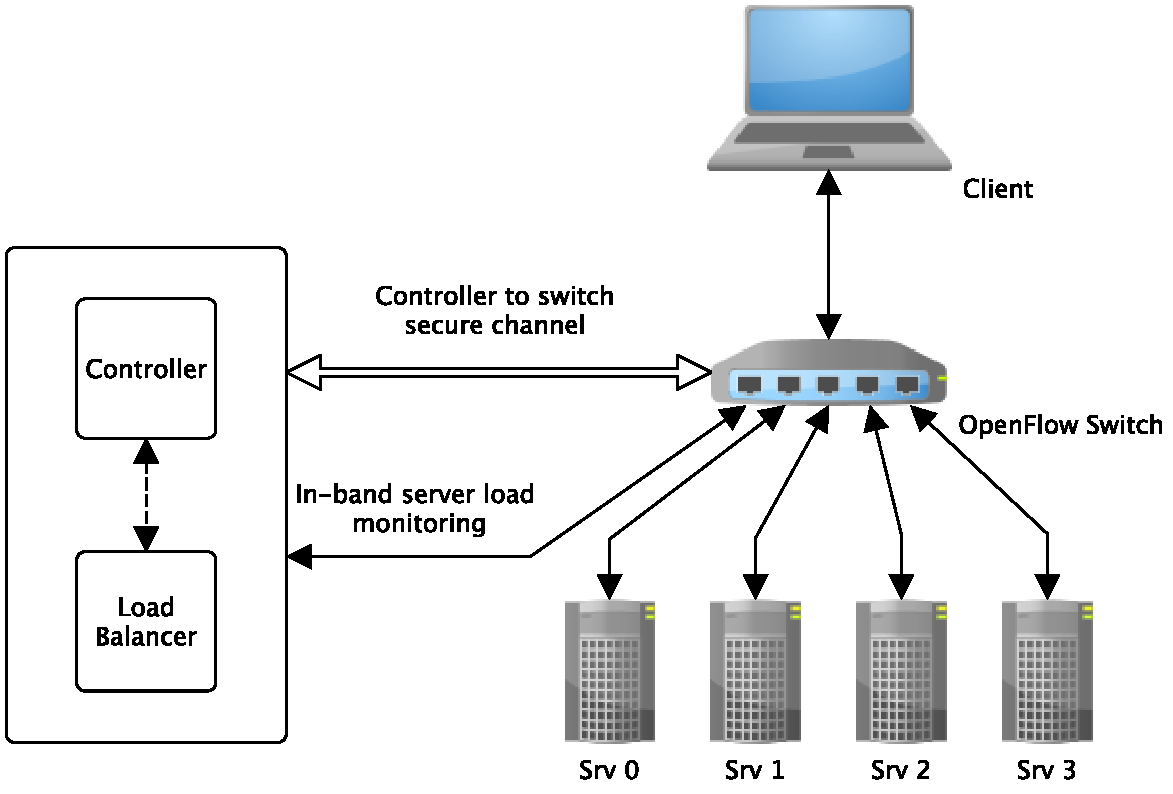
\includegraphics[scale=1.05]{img/balancer-testbed-img}
    \caption{Ambientes dos experimentos do balanceador de carga}
    \label{fig:testbed}
\end{figure}

Todos os servidores rodam o servidor web \emph{Tornado}\citep{tornado}. 
Esse servidor grava o tamanho da fila de requisições pendentes e o número de 
requisições já respondidas.


\subsection{Distribuição de carga}

Através de políticas como \emph{RoundRobin} e Aleatória, o balanceamento de 
carga distribui praticamente o mesmo número de requisições entre
os servidores.
Em políticas como Carga, Fila e Mistura a distribuição de carga é mais justa
em relação à capacidade em responder requisições por parte dos servidores.
Em um cenário heterogênio, como o presente, isso garante que a carga interna
de cada servidor seja parecida.
Por outro lado, a quantidade de requisições respondidas é diferente.
Ou seja, a distribuição é justa com o esforço nos servidores.
A figura \ref{fig:balancer-distribution} apresenta uma comparação entre as 
políticas de balanceamento de carga em um cenário com 200 conexões.

\begin{figure}[htb!]
    \centering
    \includegraphics[scale=0.7]{img/balancer-distribution.png}
    \caption{Distribuição do número de requisições por servidor. O experimento
    gerou 200 conexões com 20 requisições cada}
    \label{fig:balancer-distribution}
\end{figure}

\subsection{Justiça em relação à carga dos servidores}

A figura \ref{fig:balancer-serial-rr} apresenta o crescimento da carga nos 
servidores utilizando a política de balanceamento de carga \emph{Round Robin}.
O servidor \emph{srv102} apresenta a maior carga individual, pois respondeu
a mesma quantidade de requisições que os demais servidores.
Como pode ser visto, em um cenário onde os servidores não são iguais, existe
uma diferença considerável de carga entre os servidores.

A política \emph{RoundRobin} não é justa.
Se um servidor se sobrecarregar, ele continuará recebendo o mesmo volume de 
requisições que os demais servidores.
Esse comportamento pode gerar um aumento da taxa de perda de pacotes e uma 
redução na disponibilidade do serviço.

\begin{figure}[htb!]
    \centering
    \includegraphics[scale=0.5]{img/balancer-serial-rr}
\caption{Crescimento da carga dos servidores com o balanceador de carga 
    utilizando a política \emph{RoundRobin}. O experimento gerou 500 conexões 
        com 50 requisições cada}
    \label{fig:balancer-serial-rr}
\end{figure}


\begin{figure}[htb!]
    \centering
    \includegraphics[scale=0.5]{img/balancer-serial-load}
    \caption{Crescimento da carga dos servidores com o balanceador de carga
    utilizando a política \emph{Carga}. O experimento gerou 500 conexões com 
    50 requisições cada}
    \label{fig:balancer-serial-load}
\end{figure}

A política Carga reduz a diferença entre os servidores.
Em cada servidor a carga tende a ser mesma.
Se um servidor começar a sobrecarregar ele não será balanceado até que a 
carga reduza. 
Essa abordagem torna a distribuição de carga mais justa.
Se um servidor consegue responder mais requisições, ele 
deve receber mais requisições.
A figura \ref{fig:balancer-serial-load} mostra a distribuição mais justa 
através da política Carga.

\begin{figure}[htb!]
    \centering
    \includegraphics[scale=0.5]{img/balancer-parallel-rr}
    \caption{Crescimento da carga dos servidores utilizando a política 
    \emph{RoundRobin} com as requisições feitas em paralelo. O experimento
    gerou 500 conexões com 50 requisições em paralelo cada.}
    \label{fig:balancer-parallel-rr}
\end{figure}

\begin{figure}[htb!]
    \centering
    \includegraphics[scale=0.5]{img/balancer-parallel-load}
    \caption{Crescimento da carga dos servidores utilizando a política Carga
    com as requisições feitas em paralelo. Mesmo cenário do experimento serial}
    \label{fig:balancer-parallel-load}
\end{figure}

Esse comportamento se manteve quando os experimentos foram executados em 
paralelo utilizando \emph{httperf}.

As figuras \ref{fig:balancer-parallel-rr} e \ref{fig:balancer-parallel-load}
apresentam o resultado desses experimentos.

A política Carga distribui a carga de maneira mais justa entre os servidores.
Isso é importante em um cenário onde os servidores são heterogênios.
Toda a carga de trabalho deve ser disseminada com justiça entre os servidores.

A medição de justiça é utilizada em engenharia de redes para mostrar como 
recursos são divididos.
\emph{Jain} definiu em \citep{jain} um índice de justiça em função da 
largura de banda.
Foi adaptado o conceito do índice de justiça para considerar a carga dos 
servidores e mostrar o quão justo seria o balanceamento de carga.
A adaptação foi definida como:


\[\jmath \left ( x_1, x_2,..., x_n \right ) = \frac{\left ( \sum_{i=1}^{n} x_i\right )^2}{n \cdot \sum_{i=1}^{n} x_i^2}\]

Na avaliação de equidade/justiça de um conjunto de cargas, existem $n$
servidores e $x_i$ é a carga da amostragem.
O resultado varia de $\frac{1}{n}$ (pior caso) até $1$ (melhor caso).
O valor é máximo quando o todos os servidores recebem o mesmo número de 
alocações.
O índice é $\frac{k}{n}$ quando $k$ servidores tiveram o mesmo esforço e 
os demais $n-k$ servidores não foram escolhidos nenhuma vez. 

\begin{figure}[htb!]
    \centering
    \includegraphics[width=0.9\linewidth]{img/balancer-fairness}
    \caption{Comparação da justiça calculada para cada política de
    balanceamento de carga}
    \label{fig:fainess}
\end{figure}


\subsection{Experimento com TCP}
A largura de banda foi medida executando 15 conexões TCP de 20 segundos cada.
Todas as requisições passaram pelo balanceador de carga no controlador 
\emph{OpenFlow}.
A largura de banda foi medida a cada 5 segundos de execução do experimento.
Conforme apresentado na figura \ref{fig:balancer-tcp-bandwidth}, nota-se o 
impacto do controlador na largura de banda da rede.
A política Carga reduz a largura de banda global da rede, pois sua 
implementação demora mais para ser executada do que um simples algorítmo 
de \emph{RoundRobin}.

\begin{figure}[htb!]
    \centering
    \includegraphics[width=\linewidth]{img/balancer-tcp-bandwidth}
    \caption{Largura de banda TCP medida em 50 conexões utilizando o 
    \emph{iperf}}
    \label{fig:balancer-tcp-bandwidth}
\end{figure}

\subsection{Experimento HTTP}

A figura \ref{fig:balancer-http-full} mostra o resultado do experimento com 
5000 conexões.
O primeiro pacote de cada conexão é encaminhado para o controlador.
O controlador instala, no comutador \emph{OpenFlow}, as regras para todas 
as requisições dentro de cada conexão.

\begin{figure}[htb!]
    \centering
    \includegraphics[scale=0.5]{img/balancer-http-full}
    \caption{Experimento com 5000 conexões com 50 requisições cada}
    \label{fig:balancer-http-full}
\end{figure}

Os valores mais altos representam o atraso decorrido em função do controlador
processar os primeiros pacotes de cada conexão.
Os fluxos, para esse experimento, possuem tempo de vida (\emph{timeout}).
É importante manter a tabela de fluxos pequena e o balanceamento de carga
flexível e dinâmico.

Para compreender melhor os primeiros pacotes de cada conexão enviados para 
o controlador, a figura \ref{fig:balancer-http-zoom} mostra o experimento 
HTTP da requisição 0 até a 150.

\begin{figure}[htb!]
    \centering
    \includegraphics[scale=0.4]{img/balancer-http-zoom}
    \caption{Tempo de resposta das requisições 0 até 150}
    \label{fig:balancer-http-zoom}
\end{figure}

O primeiro pacote de cada conexão é encaminhado para o controlador.
O controlador instala um fluxo para os pacotes daquela conexão.
No controlador, para todos novoso fluxos, é instalado um fluxo reverso.
Esse fluxo representa o caminho de volta da requisição, que vai do servidor
escalonado para o cliente requisitante.
Instalar esse fluxo no comutador é importante para reduzir o número de 
pacotes entrantes (\emph{PacketIn}) que o controlador precisa lidar.

A figura \ref{fig:balancer-http-times} apresenta o tempo de resposta em segundos
de cada política de balanceamento de carga.
São apresentados os valores mínimos, máximos, médio e o desvio padrão do 
tempo de resposta das políticas.

\begin{figure}[htb!]
    \centering
    \includegraphics[width=\linewidth]{img/balancer-http-times}
    \caption{Tempo de resposta de cada política de balanceamento de carga}
    \label{fig:balancer-http-times}
\end{figure}

A política Sem Política representa requisições feitas diretamente ao servidor, 
sem passar pelo balanceador de carga.
Como pode ser visto, a média e o desvio padrão mostram que o tempo de resposta
em políticas com monitoramento é menor do que o tempo de resposta das demais
políticas.
Apesar de o controlador reduzir a largura de banda da rede, o balanceador 
de carga reduz o tempo de resposta do serviço.

\subsection{Avaliação}

O balanceador de carga não distribui o mesmo número de requisições para 
os servidores.
Fazer isso, não torna a carga bem distribuída para os servidores em um 
cenário heterogêneo. 
Considerando o esforço de cada servidor como o parâmetro de justiça, a solução
de balanceamento de carga proposto distribui de maneira mais justa a carga 
entre os servidores de aplicação.
A carga dos servidores cresce de maneira homogênea.

Como pode ser visto na figura \ref{fig:balancer-tcp-bandwidth}, pacotes 
encaminhados para o controlador impactam a largura de banda da rede.
No entanto, a solução de balanceamento de carga reduz o tempo de resposta 
do serviço. 
Os fluxos reversos são uma estratégia inteligente que instala fluxos no 
comutador antes de eles saírem do servidor.

Esse capítulo apresentou uma breve avaliação do \emph{OpenFlow} aplicado 
a um sistema de balanceamento de carga.
Os próximos capítulos irão abordar a solução e os resultados obtidos para
a proposta de um módulo em grafos para o controlador.
